\documentclass[11pt]{amsbook}

\usepackage{../HBSuerDemir}	% ------------------------


\begin{document}

% ++++++++++++++++++++++++++++++++++++++
\hPage{b1p2/372}
% ++++++++++++++++++++++++++++++++++++++

\begin{exmp}
	\begin{hSolution}
		\begin{hEnumerateArabic}
			
			\item
			\begin{multicols}{2}
				By rectangular rule:
				\begin{align*}
					A & \cong h( \frac{3}{4} + \frac{3}{5} + \frac{1}{2} 
						+ \frac{3}{7} + \frac{3}{8} + \frac{1}{3}) \\
					& = \frac{1}{3} (0,750+0,600+0,500+0,429+0,375+0,333) \\
					& = \frac{1}{3} \times 2,987 = \underline{0,996} \quad \text{(lower sum)} \\
					A & = h(1,000+0,750+0,600+0,500+0,429+0,375) \\
					& = \frac{1}{3} \times 3,654 = \underline{1,218} \quad \text{(upper sum)}
				\end{align*}
			
				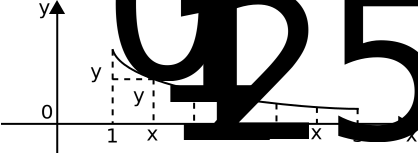
\includegraphics[width=0.35\textwidth]{images/b1p2-372-fig01}
				\footnote{Corrected the figure: In the question in previous page the integral is from 1 to 3 but in the figure it is from 1 to 6}
			\end{multicols}

			The average of these two results is \underline{1,107}.
			
			\item
			\begin{align*}
				A & = \frac{h}{2} (1+2 \times 0,750 + 2 \times 0,600 + 2 \times 0,500 + 2\times 0,429
					+ 2 \times 0,375 + 0,333) \\
				& = \frac{1}{6} \times 6,641 = \underline{1,107}
			\end{align*}
			
			\item
			By Simpson's rule: It is applicable since n is even.
			\begin{align*}
				A & = \frac{h}{3} (1 + 4 \times 0,750 + 2 \times 0,600 + 4 \times 0,500 + 2 \times 0,429
					+ 4 \times 0,375 + 0,333) \\
				& = \frac{1}{9} \times 9,791 = \underline{1,088} \quad \text{Then } \ln 3 \cong 1,088.
			\end{align*}
			In the same way $\ln 2$ can be computed and one gets
			\[
				\ln 2 = \int_{1}^{2} \frac{\hDif x}{x} \cong \underline{0,69}
			\]
		\end{hEnumerateArabic}
	\end{hSolution}
\end{exmp}

\begin{exmp}
	For the function given in tabular form
	\begin{center}
		\begin{tabular}{c|ccccc}
			$x_{i}$ & 0 & 1/4 & 1/2 & 3/4 & 1 \\
			\hline
			$f(x_{i})$ & 1 & 17/16 & 5/4 & 25/16 & 2
		\end{tabular}
	\end{center}
	evaluate the definite integral
	\[
		B = \int_{0}^{1} f(x) \, \hDif x
	\]
	approximately by SIMPSON's rule with n necessarily equal to 2 or 4.
	
	\begin{hSolution}
		Taking $n=4$, we have $h=1/4$, and
		\begin{align*}
			B & = \frac{1}{12} ( 1,000+4\times\frac{17}{16} + 2 \times \frac{5}{4} + 4 \times \frac{25}{16}+2)\\
			& = \frac{1}{12} \times 16,000 = \underline{1,333}
		\end{align*}
		\footnote{The place of the bracket corrected. B=(1/12... to B=1/12(...}
	\end{hSolution}
\end{exmp}
Note: When a function is given in tabular form and $x_{i}-x_{i+1}$


% =======================================================
\end{document}  